\documentclass[aspectratio=169]{beamer}
% \RequirePackage[T2A]{fontenc}
\RequirePackage[utf8]{inputenc}
%\RequirePackage[english,russian]{babel}

\usepackage{listings}
\usepackage{courier}
\usepackage{tikz}
\usepackage{float}
\usepackage{graphicx}
\usepackage{epstopdf}

\usepackage{algorithm2e}

 % Перевод плагина
\SetKwInput{KwData}{Input parameters}
\SetKwInput{KwResult}{Result}
\SetKwInput{KwIn}{Input data}
\SetKwInput{KwOut}{Output Data}
\SetKwIF{If}{ElseIf}{Else}{if}{then}{else\ if}{else}{end\ of\ condition}
\SetKwFor{While}{while}{execute}{end\ of\ loop}
\SetKw{KwTo}{to}
\SetKw{KwRet}{return}
\SetKw{Return}{return}
\SetKwBlock{Begin}{begin\ block}{end\ block}
\SetKwSwitch{Switch}{Case}{Other}{Check\ a\ value}{and\ execute}{a\ case}{otherwise}{end\ of\ case}{end\ of\ value\ check}
\SetKwFor{For}{loop}{execute}{end\ of\ loop}
\SetKwFor{ForEach}{for\ each}{execute}{end\ of\ loop}
\SetKwRepeat{Repeat}{repeat}{while}
\SetAlgorithmName{Algorithm}{algorithm}{List of algorithms}


\usetikzlibrary{shapes,arrows}

%\usetheme{CambridgeUS}%{Warsaw}
%\usetheme {Madrid}
%\useoutertheme {shadow}
%\usecolortheme{beaver}%{structure черный}%{seagull серый}%{lily желтый}%{beaver красный}
%\usefonttheme{structurebold}
%\setbeamerfont{framesubtitle}{size=\large}
%\useoutertheme{infolines}
%\useoutertheme{split}
%I DONT WANT TO SEE THOSE NAVIGATION SYMBOLS
%\setbeamertemplate{navigation symbols}{}

\mode<presentation>
{
    \usefonttheme[onlymath]{serif}
\usetheme {Madrid}
%\useoutertheme {shadow}
%\usecolortheme{beaver}%{structure черный}%{seagull серый}%{lily желтый}%{beaver красный}
\usefonttheme{structurebold}
\setbeamerfont{framesubtitle}{size=\large}
\useoutertheme{infolines}
%\useoutertheme{split}
%I DONT WANT TO SEE THOSE NAVIGATION SYMBOLS
\setbeamertemplate{navigation symbols}{}
\setbeamertemplate{footline}
}

\setbeamercolor{color1}{bg=red!40!green,fg=black}
\setbeamercolor{uppercol}{fg=white,bg=brown}

\usepackage{iftex,ifxetex}
\ifPDFTeX
  \usepackage[utf8]{inputenc}
  %\usepackage[T1]{fontenc}
  %\usepackage[russian]{babel}
  \usepackage{lmodern}
  \usefonttheme{serif}
\else
  \ifluatex
    \usepackage{unicode-math}
    \defaultfontfeatures{Ligatures=TeX,Numbers=OldStyle}
    \setmathfont{Latin Modern Math}
    \setsansfont{Linux Biolinum O}
    \usefonttheme{professionalfonts}
    \setmathfont[
        Ligatures=TeX,
        Scale=MatchLowercase,
        math-style=upright,
        vargreek-shape=unicode
        ]{euler.otf}
  \fi
\fi


\title{Control Flow Graph Visualization in\\ Compiled Software Engineering}

\author[A.~Mikhailov]{\textbf{Andrey Mikhailov}${}^{*}$, \textbf{Aleksey Hmelnov}${}^{*}$, \\\underline{Evgeny Cherkashin}${}^{*\;**}$, Igor Bychkov${}^{*}$\\\texttt{\scriptsize{\{mikhailov,alex,eugeneai,bychkov\}@icc.ru}}}


\institute[ISDCT SB RAS, INRTU]
{${}^{*}$Matrosov Institute for System Dynamics and Control Theory of Siberian Branch of Russian Academy of Sciences; \\[0.5em]
${}^{**}$Irkutsk National Research Technical University,\\
Irkutsk, Russian Federation\\[0.7cm]
}

\date{\scriptsize{
\\
    \vspace{0.3cm}}
ISDCT SB RAS, INRTU
\\
31 May 2016
\\
Opatija, Croatia
}
\begin{document}

%\титульный
%\section{Delphi}
\maketitle

%\граф потоков управления

\begin{frame}
  \frametitle{Applications}
  Control flow graph (CFG) analysis is a common stage in syntactic approaches of data mining and pattern recognition, e.g., in source and binary code analysis in software and instrumental tool quality assessment:
  \begin{itemize}
  \item compiled binary code productivity;
  \item quality of compiler and system libraries;
  \item features of hardware platforms;
  \end{itemize}
Also CFG is used as a pattern recognition technique in
  \begin{itemize}
  \item reconstruction of legacy source code;
  \item malware and virus code analysis;
  \item Model Driven Engineering software development.
  \end{itemize}
\end{frame}

%\section{Delphi}
\begin{frame}
\frametitle{Control flow graph}

\newtheorem{Def}{Definition}[section]
\begin{Def}
An directed graph $G(V,E)$ is a \textbf{control flow graph} if the following holds:
\begin{enumerate}
\item graph $G$ does not contain multiple edges;
\item node $start\in V$ is the only entrance to the graph;
\item node $end \in V$ is the exit from the graph;
\item each node $v \in V$ is accessible from $start$;
\item node $end$ is accessible from each node $v \in V$.
\end{enumerate}
%If a control flow graph has more than one terminal node, the terminal nodes are connected to one new fictitious terminal node.
\end{Def}

\newtheorem{DOM}{Definition}[section]
\begin{Def}
A node $x$ is a \textbf{dominator} of $y$ ($x\quad dom\quad y$) in a directed graph, if any path from $start$ to $y$ includes $x$.
\end{Def}

\newtheorem{IDOM}{Definition}[section]
\begin{Def}
A node $x$ is an \textbf{immediate dominator} of $y$ ($x\quad idom\quad y$), if $x\quad dom\quad y$ and there are no such $p$ that $x\quad dom\quad p$ and $p\quad dom\quad y$.
\end{Def}

%A node $x$ is a \emph{postdominator} of $y$ ($x\quad pdom\quad y$), if any path from $y$ to $end$ includes $x$.  By convention, a node dominates and postdominates itself.    A node $x$ is an \emph{immediate postdominator} of $y$ ($x\quad pidom\quad y$), if $x\quad pdom\quad y$ and there are no such $p$ that $x\quad pdom\quad p$ and $p\quad pdom\quad y$.

\end{frame}

%\ иерархический раскладчик

%\section{Delphi}
\begin{frame}
\frametitle{Hierarchic layout engine}
\textbf{Software:} uDraw (daVinci), VCG, Graphlet, GraVis, Graph Drawing Server, graphViz, VisualGraph.
\begin{enumerate}
\item \textbf{Distribution of graph nodes between layers.} Each node is assigned a rank.  All directed edges can connect nodes from a lower rank to a higher one.  Rank distribution of the nodes is performed, \emph{e.g.}, on the base of path length calculation in depth-first graph traversal procedure.
\item \textbf{Defining order on the nodes in a layer.} The nodes of a layer are ordered according to principle of minimization of intersections of edges, e.g., by means of Method of median.
\item \textbf{Figuring out of the node coordinates in a layer.} Each node of each layer is assigned a coordinate so as the graph will correspond to predefined aesthetic criteria.
\item \textbf{Edge drawing.} The edges are drawn according to rules of visualization, for example, as arrows.
\end{enumerate}
\end{frame}

%\критерии качества визуализации

%\section{Delphi}
\begin{frame}
\frametitle{Quality criteria of graph visualization}

%	\newtheorem{vis}{Definition}
%	\begin{vis}
A display of the nodes and the edges of a graph on a surface (or in a 3d-space) is referred to as a \emph{graph layout}.
%	\end{vis}

	\begin{itemize}
\item \textbf{Visual arrangement} is the main set of rules that a graph representation must obey to be acceptable as a desired result, \textit{e.g.}, to visualize programs as a flowchart, the rules of flowchart layout is used.
\item \textbf{Aesthetics} is a subset of the criteria that defines attributes of the constructed image, \textbf{improving visual quality}.
\item \textbf{Restrictions} are a subset of the criteria that define layout rules for specific elements and subgraphs of the constructed image, \textit{e.g.}, place root at the center of image, place nodes outside of a region.
\end{itemize}
	\begin{figure}[htbp]
		\centering
			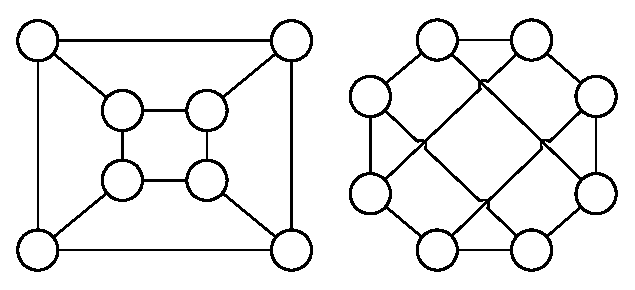
\includegraphics[width=0.40\textwidth]{Pic/Pic1.eps}
                \caption{Various layouts of the same graph}
		\label{fig:VisExample}
	\end{figure}
\end{frame}

%\изобразительные соглашения

%\section{Delphi}
\begin{frame}
\frametitle{Visual arrangements for flowcharts}
\begin{enumerate}
\item [a)]\textbf{Operator shape} represents a node where the control flow passed only one direction.
\item [b)]\textbf{Branching shape} corresponds to conditional operators in high-level programming languages; in a control flow graph it is a node, where flow control splits up.
\item [c)]\textbf{Cycle edge shapes} denote two graph nodes, one is for beginning of the cycle and one for its end, the cycle body is located between these shapes.
\item [d)]\textbf{Starting and terminal shapes} mark the entrance and the exit from a function or a program.
	\end{enumerate}

\begin{figure}[htbp]
  \begin{minipage}[b]{0.24\linewidth}
    \center{
\includegraphics[width=0.35\textwidth]{Pic/BlocksA.eps} \\ \footnotesize\emph{a})\\ operator}
  \end{minipage}
  \hfill
  \begin{minipage}[b]{0.24\linewidth}
    \center{
\includegraphics[width=0.35\textwidth]{Pic/BlocksB.eps} \\ \footnotesize\emph{b})\\ branching}
  \end{minipage}
  \begin{minipage}[b]{0.24\linewidth}
    \center{
\includegraphics[width=0.5\textwidth]{Pic/BlocksC.eps} \\ \footnotesize\emph{c})\\ cycle edges}
  \end{minipage}
  \begin{minipage}[b]{0.24\linewidth}
    \center{
\includegraphics[width=0.35\textwidth]{Pic/BlocksD.eps} \\ \footnotesize\emph{d})\\ start/termination}
  \end{minipage}
\end{figure}
\end{frame}

%\TT регион

%\section{Delphi}
\begin{frame}
\frametitle{Two terminal (TT) region}

\newtheorem{TT}{Definition}[section]
\begin{Def}
A subgraph having one entry and one exit node is a \emph{TT region}.

A node pair $\langle a, b\rangle$ of a graph $G$ is a TT region if
	\begin{enumerate}
		\item[1)]
			$a$ idom $b$;
		\item[2)]
			$b$ postidom $a$;
		\item[3)]
			any graph cycle containing $a$ also contains $b$ and vice versa.
	\end{enumerate}
\end{Def}


\begin{figure}[htbp]
	\centering
		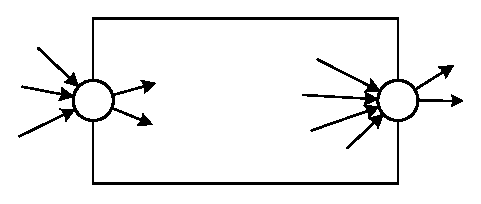
\includegraphics[width=0.5\textwidth]{Pic/TTRegion.eps}
	\caption{A two terminal region}
	\label{fig:TTRegion}
\end{figure}

\end{frame}

%\выделяемые регионы

%\section{Delphi}
\begin{frame}
\frametitle{Recognizable regions}
\begin{figure}[htbp]
	\centering
		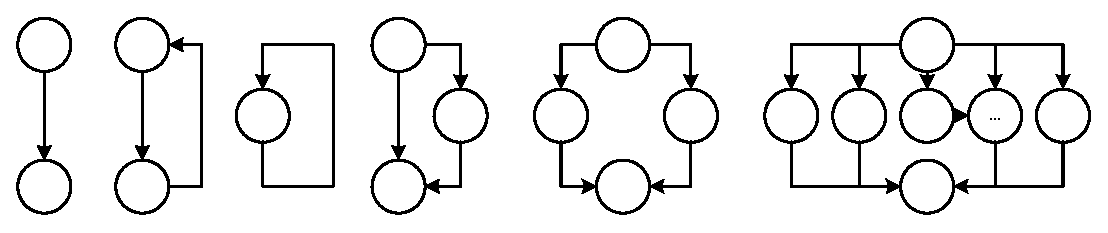
\includegraphics[width=1\textwidth]{Pic/Reg.eps}
	\caption{Patterns of regions}
	\label{fig:Regions}
\end{figure}
\end{frame}

%\алгоритм структурирования

%\section{Delphi}
\begin{frame}
\frametitle{Algorithm of control flow graph structuring}
\small{%
\begin{algorithm}[H]
\SetAlgoLined %% Connects logical parts with lines
\KwData{G, D, P}
\KwResult{An abstract node containing a hierarchy of folded subgraphs}
%\While{$|E| \neq 0$ и $|V| \neq 1$}{
	\ForEach{$v \in D$ in a backward breadth-first order}{
		\ForEach{$p \in Children(v)$}{
			\If{$p\quad pidom\quad v$}{
				$S \leftarrow Children(v) \setminus p $ \\
				\If{$Classify\_Region(S) \neq \textit{undeterminated}$}{
					$Apply\_Template(S)$
				}\Else{
					$Hierarchical\_Layout(S \cup p)$ \\
					$Recognize\_Undeterminanted\_Region(S)$
				}
				$Modify(G,D,P)$
			}
		}
	}
%}
\end{algorithm}%
}
\end{frame}

%\Визуализация

%\section{Delphi}
\begin{frame}
\frametitle{Layout procedure}

The layout process is a top-down recursive procedure of region recognition and visualization.  For the top region the initial coordinates are specified.

\begin{figure}[htbp]
	\centering
		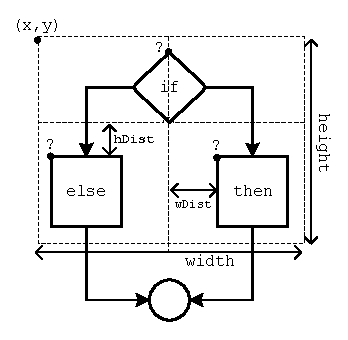
\includegraphics[width=0.4\textwidth]{Pic/IfThenElse.eps}
	%\caption{pattern of \texttt{if-then-else} operator}
	\label{fig:IfThenElse}
\end{figure}

\end{frame}

%\Результат раскладки

%\section{Delphi}
\begin{frame}
\frametitle{A layout example of a control flow graph}
\begin{figure}[htbp]
	\begin{minipage}[t]{0.45\linewidth}
	\center{
%\includegraphics[width=0.5\textwidth]{Pic/Hgraph.pdf} \\
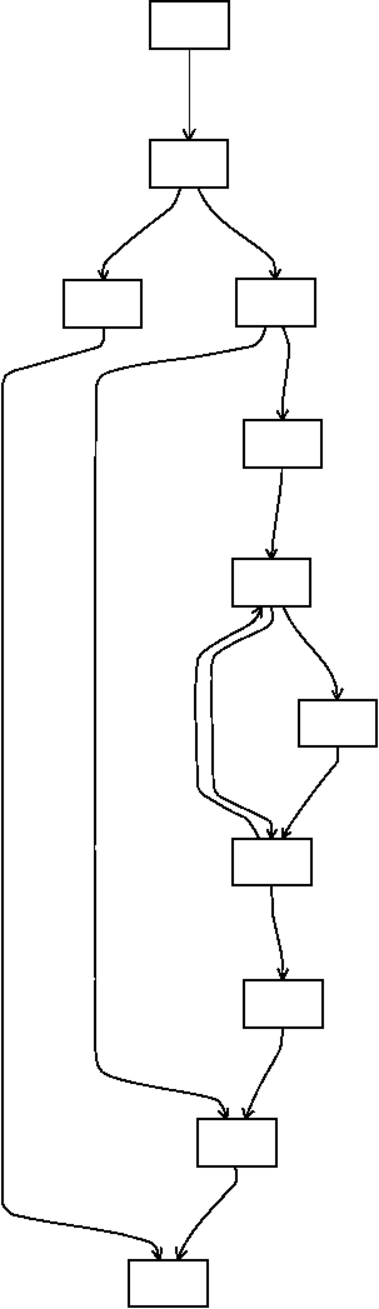
\includegraphics[width=0.3\textwidth]{Pic/Hier.pdf}
a) Hierarchical layout}
	\end{minipage}
\hfill
\begin{minipage}[t]{0.49\linewidth}
	\center{\includegraphics[width=0.44\textwidth]{Pic/Sgraph.pdf} b) Structural layout}
	\end{minipage}
\end{figure}
\end{frame}

%\Тестирование

%\section{Delphi}
\begin{frame}
\frametitle{Testing results}
\begin{itemize}
	\item 197.parser\footnote{Syntactic parsing for natural language}
	\item 252.eon\footnote{Ray tracing}
\end{itemize}

About 70\% of graphs are structured completely \textbf{without undeterminanted} regions.  Around 96\% of recognized regions are structured.

Main advantages of the approach:
\begin{itemize}
	\item Visual arrangement rule set change by means of new templates.
	\item Similar visualization for the same operators of different programming languages.
	\item The possibility to emphasize graph regions according to a recognized semantics.
\end{itemize}

\end{frame}
\maketitle
\end{document}

%%% Local Variables:
%%% mode: latex
%%% TeX-master: t
%%% End:
